% !TeX root = ../../thesis.tex
\chapter{Applications: Mechanical integrity of infilled structures}\label{ch:infill}

\section{Introduction}

\section{Methods}

\begin{figure}[h]
\centering
\medskip
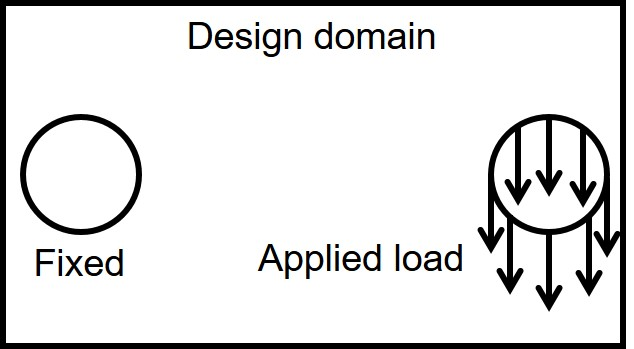
\includegraphics[width=0.5\textwidth]{domain.jpg}
\caption[Computational domain for the topology optimization]{Computational domain for the topology optimization} \label{fig:infill_domain}
\end{figure}


\begin{figure}[h]
\centering
\medskip
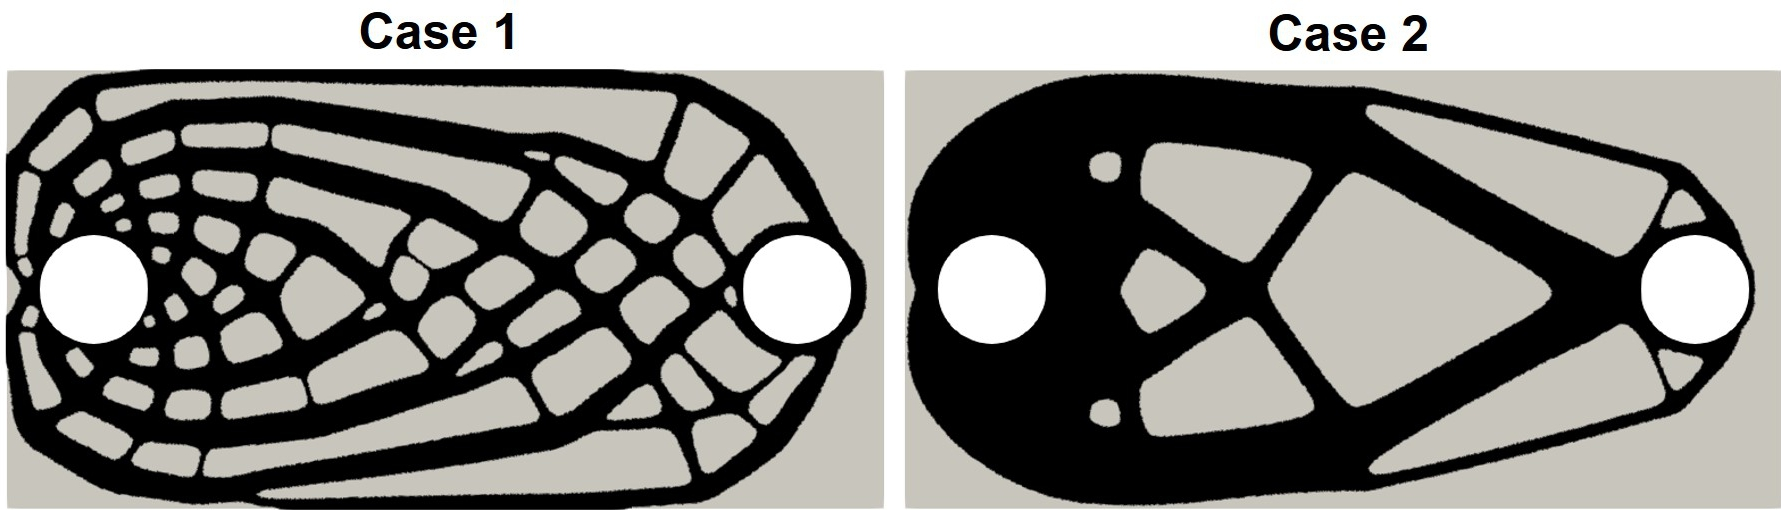
\includegraphics[width=\textwidth]{final_cases.jpg}
\caption[Topology optimization output to be used in the biodegradation simulations]{Topology optimization output to be used in the biodegradation simulations} \label{fig:infill_final_cases}
\end{figure}


\begin{figure}[h]
\centering
\medskip
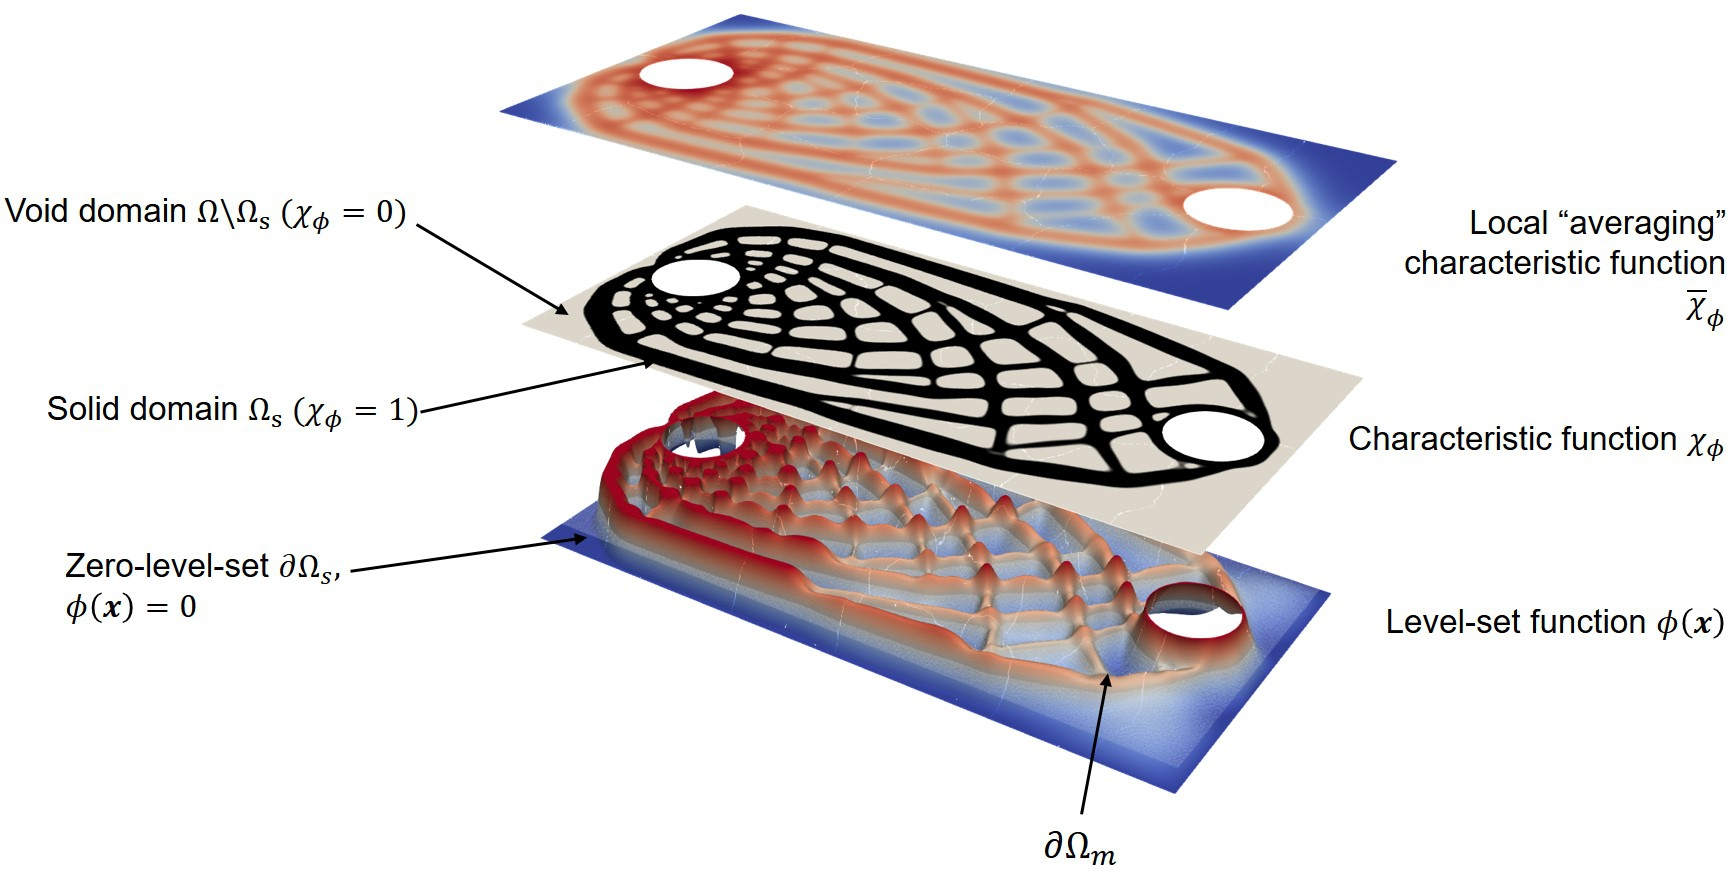
\includegraphics[width=\textwidth]{diagram.jpg}
\caption[Coupling topology optimization and biodegradation models]{Coupling topology optimization and biodegradation models} \label{fig:infill_diagram}
\end{figure}


\begin{figure}[h]
\centering
\medskip
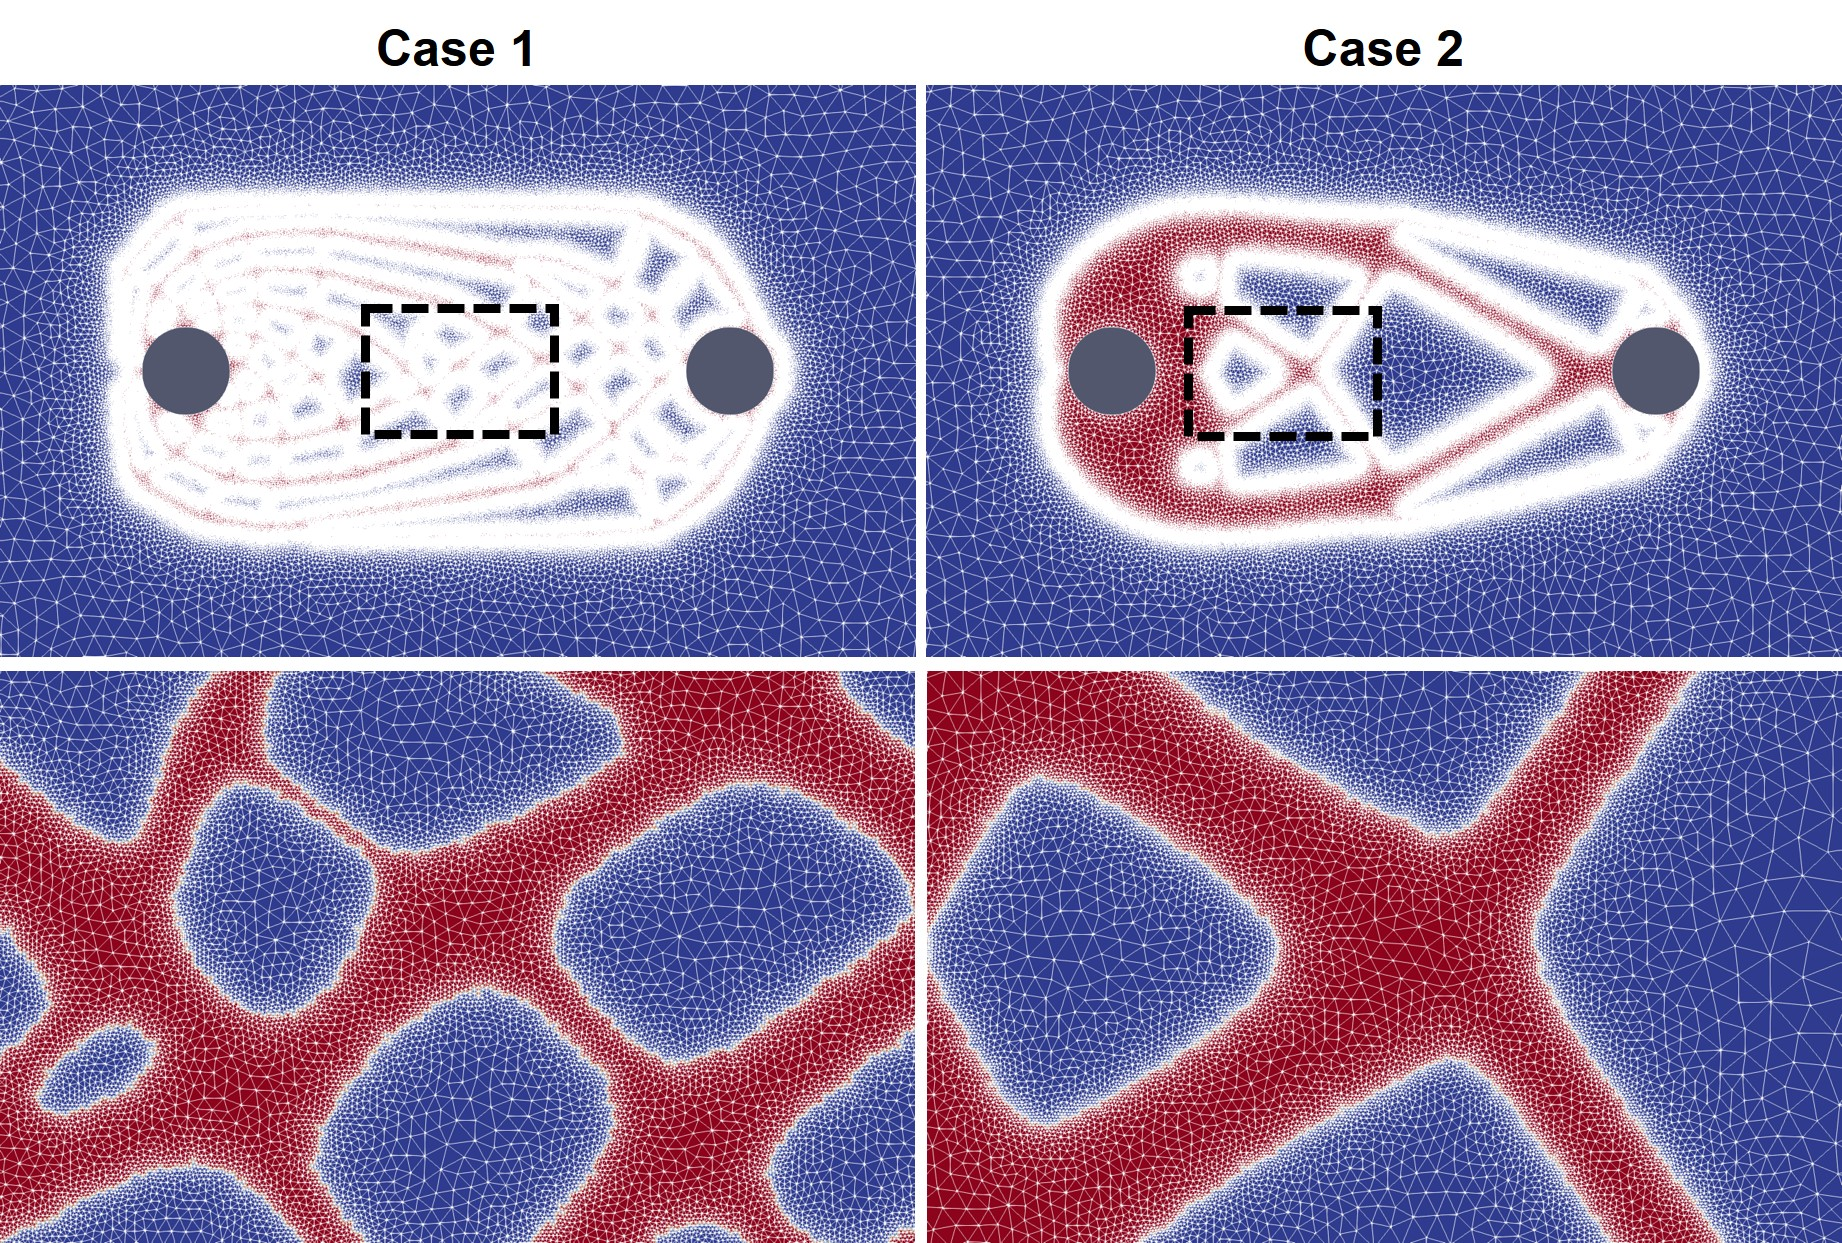
\includegraphics[width=\textwidth]{mesh.jpg}
\caption[Computational mesh for the biodegradation simulations]{Computational mesh for the biodegradation simulations} \label{fig:infill_mesh}
\end{figure}



\section{Results}

The coupled biodegradation and structural mechanics models were constructed using the output of the TO procedure. Fig. \ref{fig:infill_case1_to_steps} shows the temporary evolving shapes of the infill during the optimization process for case 1, each of which is taken by skipping 40 intermediate steps. Fig. \ref{fig:infill_case2_to_steps} shows a similar 2D visualization for case 2.


\begin{figure}[h]
\centering
\medskip
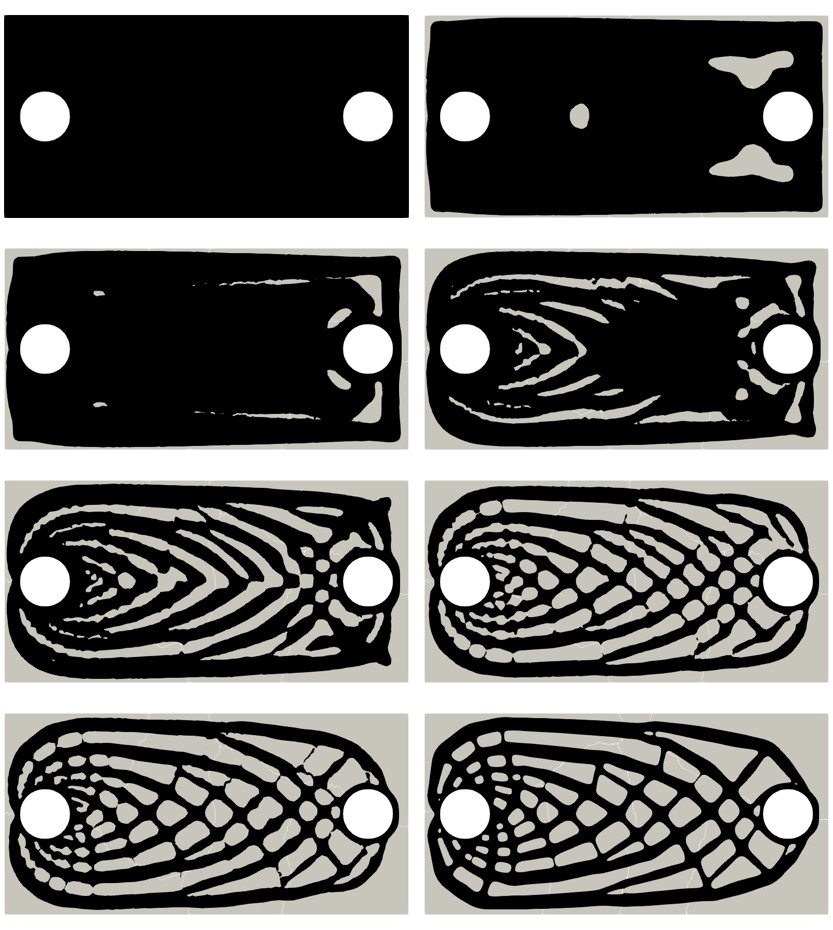
\includegraphics[width=\textwidth]{case1_to_steps.jpg}
\caption[Evolution of the topology optimization level set function for case 1]{Evolution of the topology optimization level set function to get the optimized shape for case 1, in which a local volume constraint was imposed.} \label{fig:infill_case1_to_steps}
\end{figure}

\begin{figure}[h]
\centering
\medskip
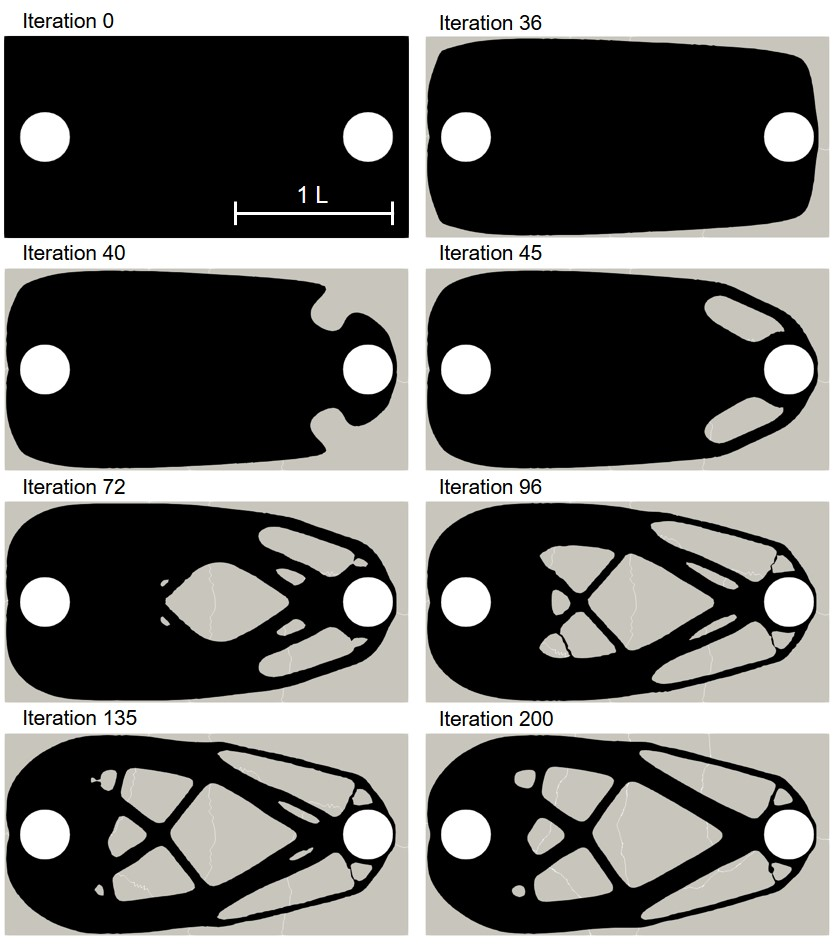
\includegraphics[width=\textwidth]{case2_to_steps.jpg}
\caption[Evolution of the topology optimization level set function for case 2]{Evolution of the topology optimization level set function to get the optimized shape for case 1, where only the global volume constraint was imposed.} \label{fig:infill_case2_to_steps}
\end{figure}

Fig. \ref{fig:infill_degradation_stiffness} shows the quantitative results of both components of the coupled computational model for the investigated cases. On the top row, the degradation rate is plotted by measuring the mass loss over time, showing how the diffusion rate of the Mg ions affects the rate of biodegradation in this model. On the bottom row, the change of the stiffness during the biodegradation is plotted, where the stiffness is calculated by inverting the compliance, the objective function of the TO routine calculated in each time step after adjusting the geometry in presence of degradation.


\begin{figure}[h]
\centering
\medskip
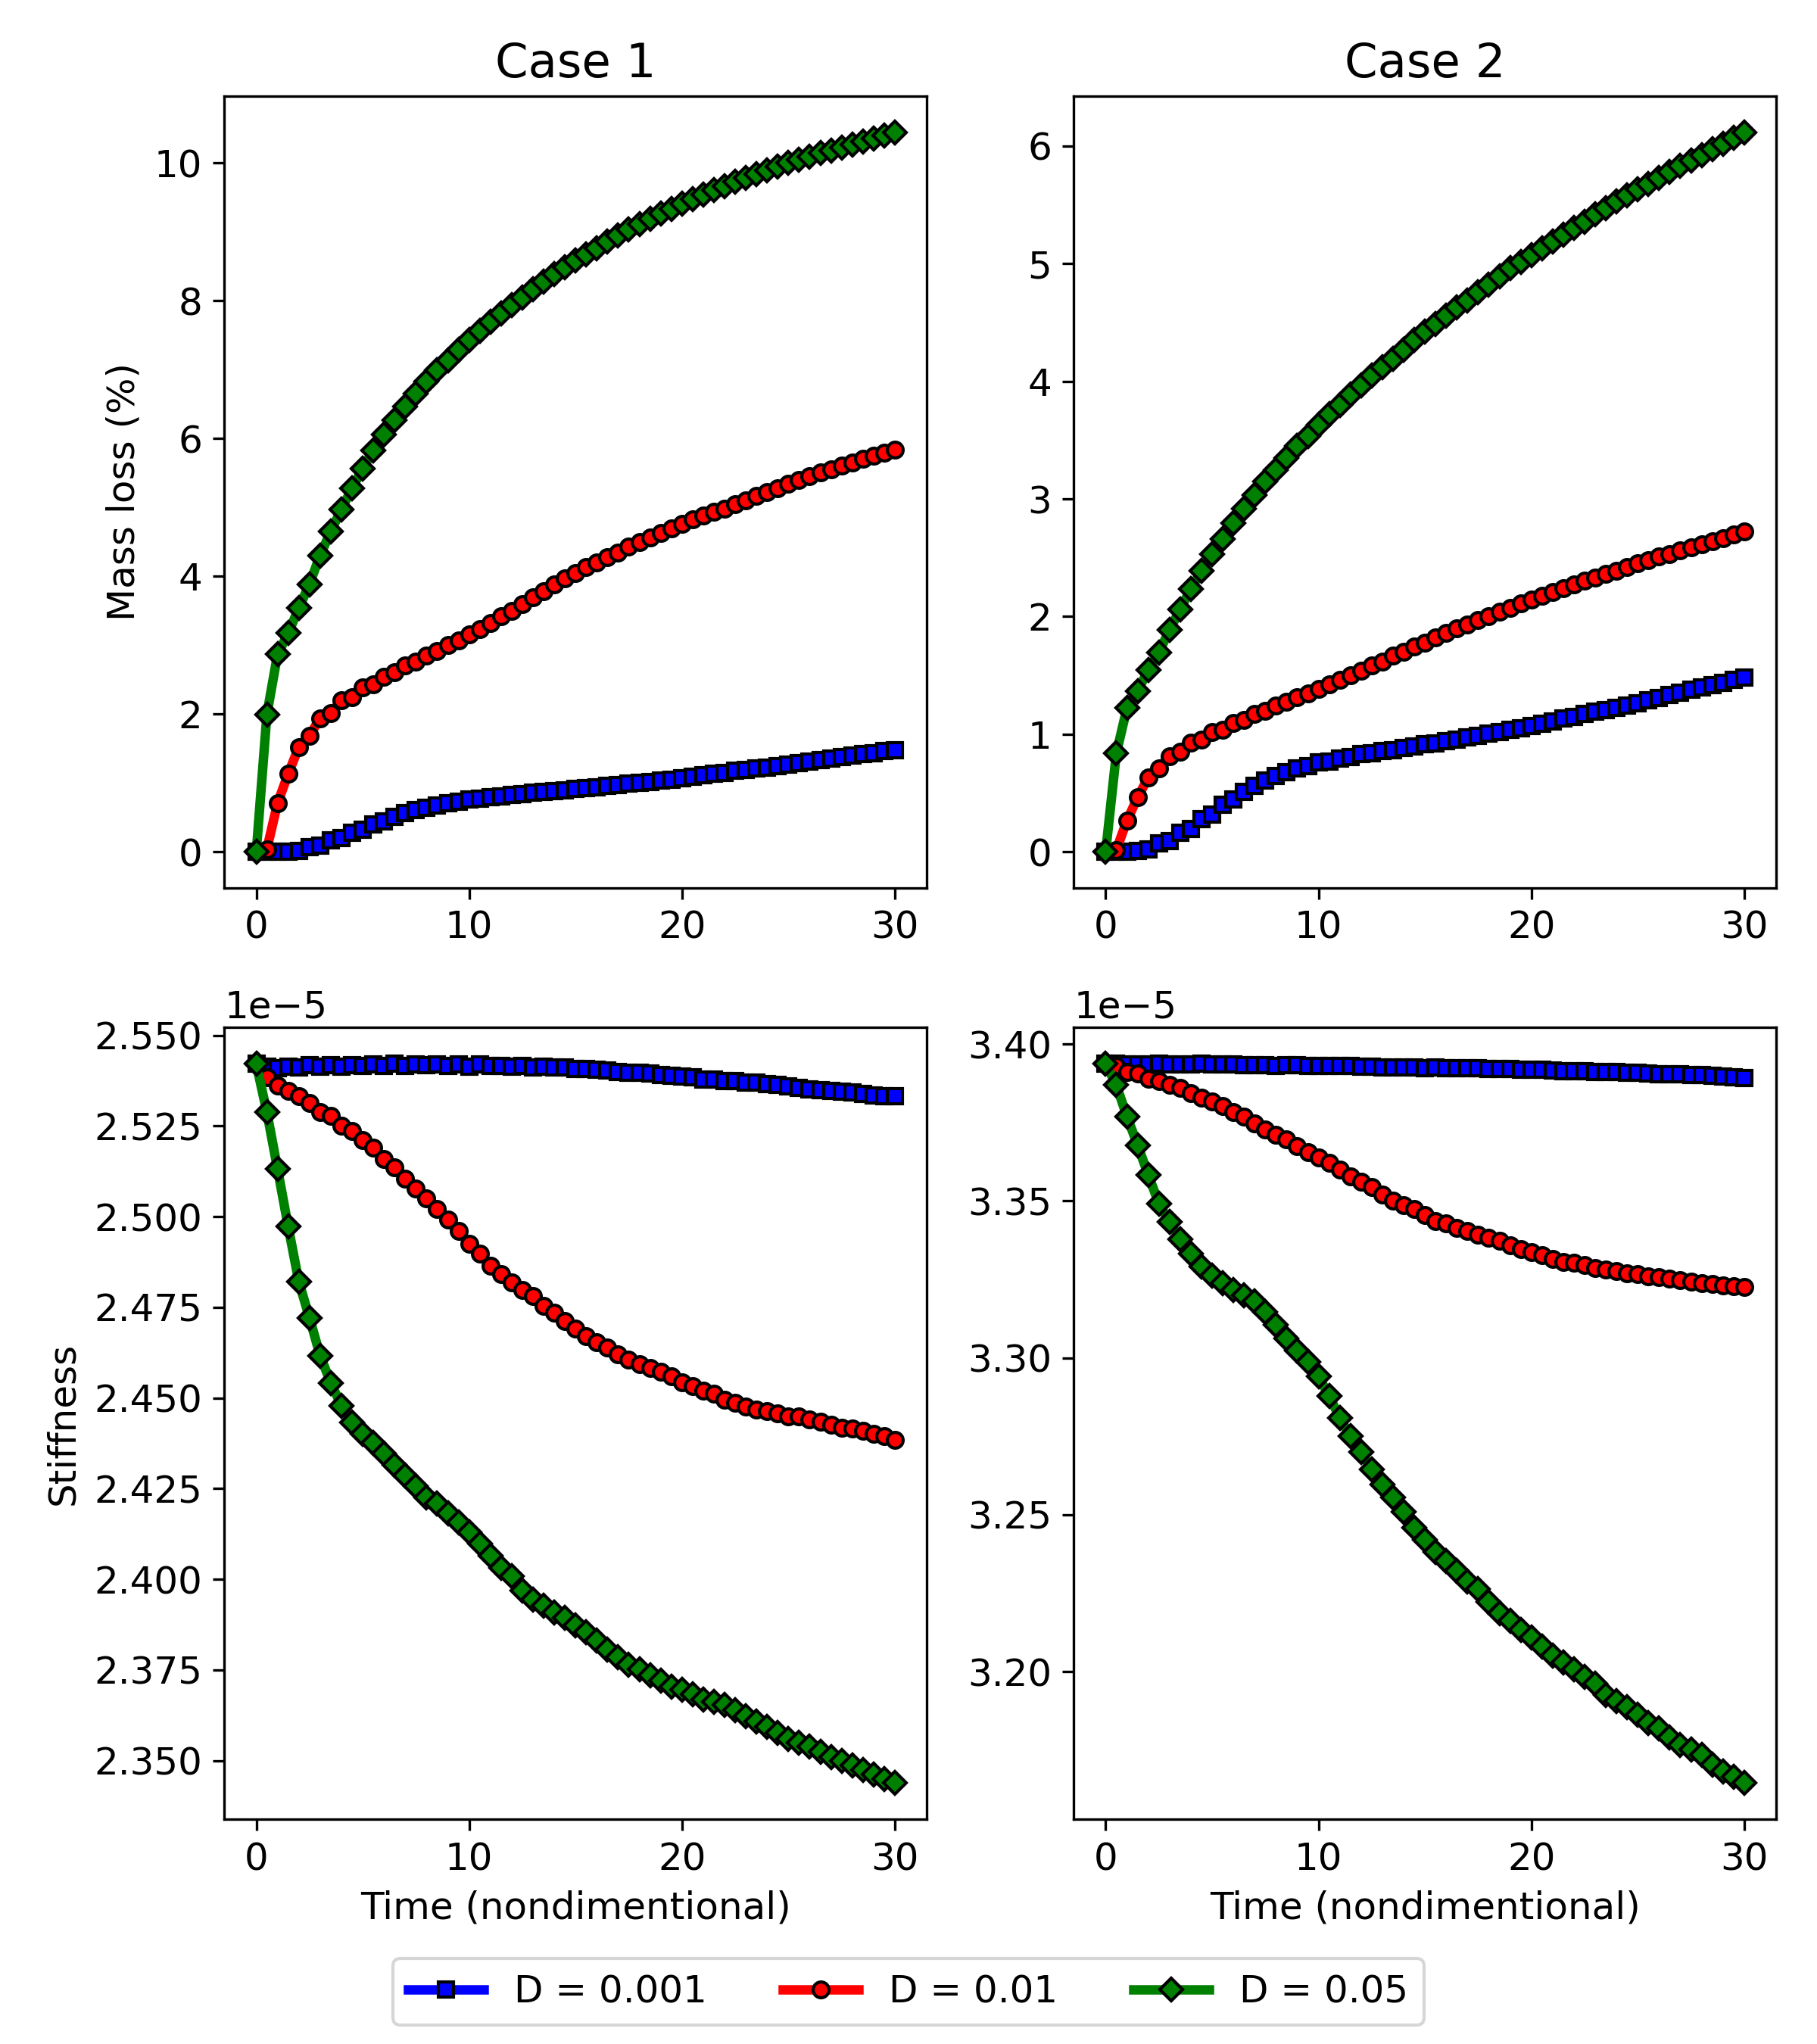
\includegraphics[width=\textwidth]{degradation_stiffness.png}
\caption[Results of the coupled model to predict the stiffness changes during biodegradation]{Results of the coupled model to predict the mass loss and stiffness changes during the biodegradation process of the infilled shapes.} \label{fig:infill_degradation_stiffness}
\end{figure}

Fig. \ref{fig:infill_results_mechanics} demonstrate how the qualitative results of the coupled model look like, in which the infilled part goes under the degradation and mechanical load at the same time. The green surface is the result of the mechanical analysis, visualized by bending the part according to the computed deformation vector in each node. The light green surface is the degradation object without bending being visualized, showing the change of the morphology due to biodegradation while the release of the metallic ions are also depicted.


\begin{figure}[h]
\centering
\medskip
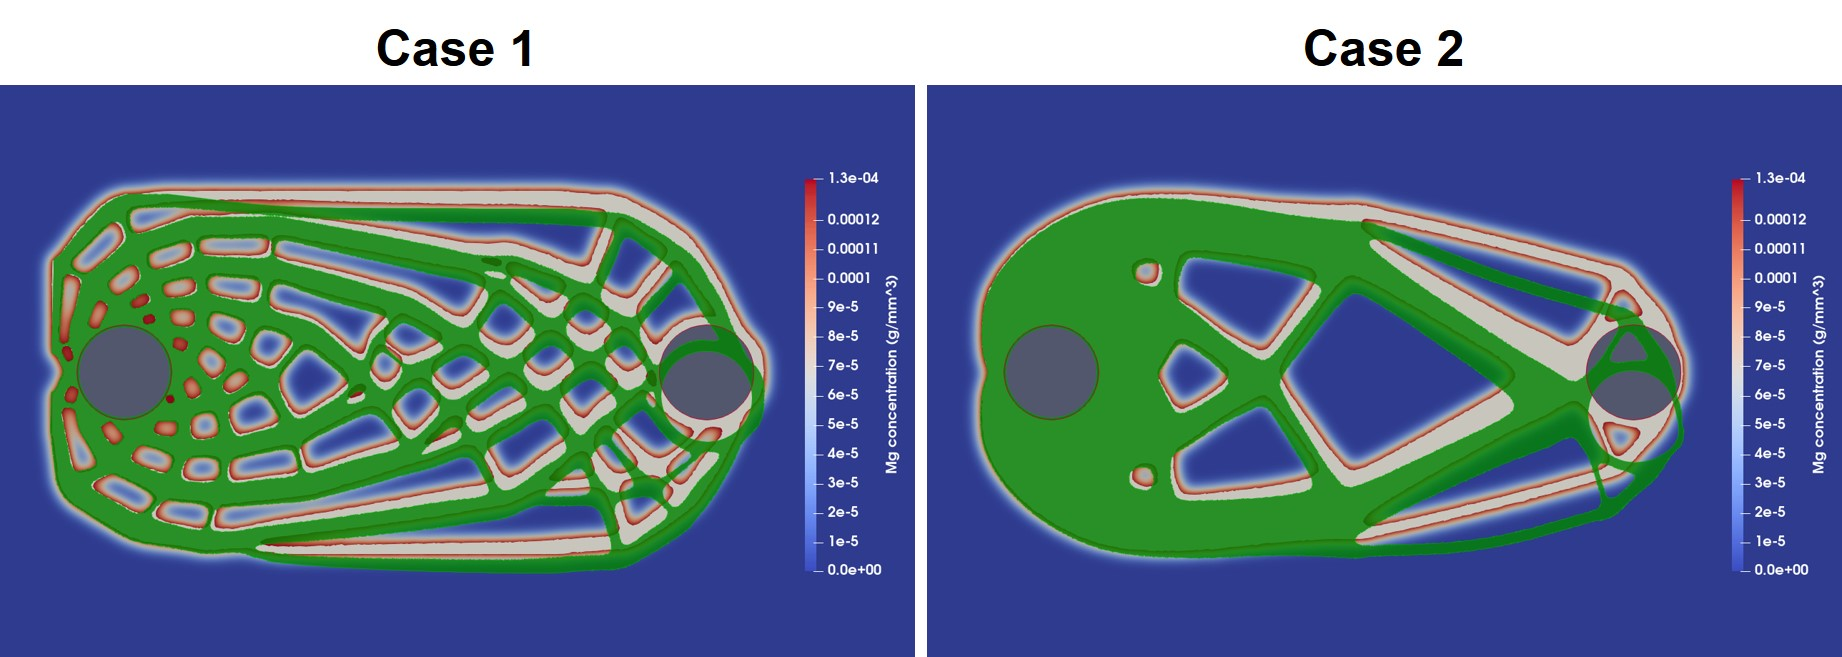
\includegraphics[width=\textwidth]{results_mechanics.jpg}
\caption[Coupled model results showing the stiffness analysis taking place during biodegradation simulation]{Coupled model results showing the stiffness analysis taking place during the biodegradation simulation. The green surface shows the deformed infilled structure, and the light gray surface is the state of the morphology during biodegradation. The colors show the concentration of metallic ions as being released from the surface of the degrading part.} \label{fig:infill_results_mechanics}
\end{figure}

In order to visualize the biodegradation only, the green surface is removed from Fig. \ref{fig:infill_results_mechanics}, and the results are plotted in various time points during the process. Figs. \ref{fig:infill_results_degradation_case1} and \ref{fig:infill_results_degradation_case2} show such visualization for case 1 and case 2, respectively, in which the surface of the degrading part is depicted in light gray, showing how the metallic ions are released during the biodegradation process. 

\begin{figure}[h]
\centering
\medskip
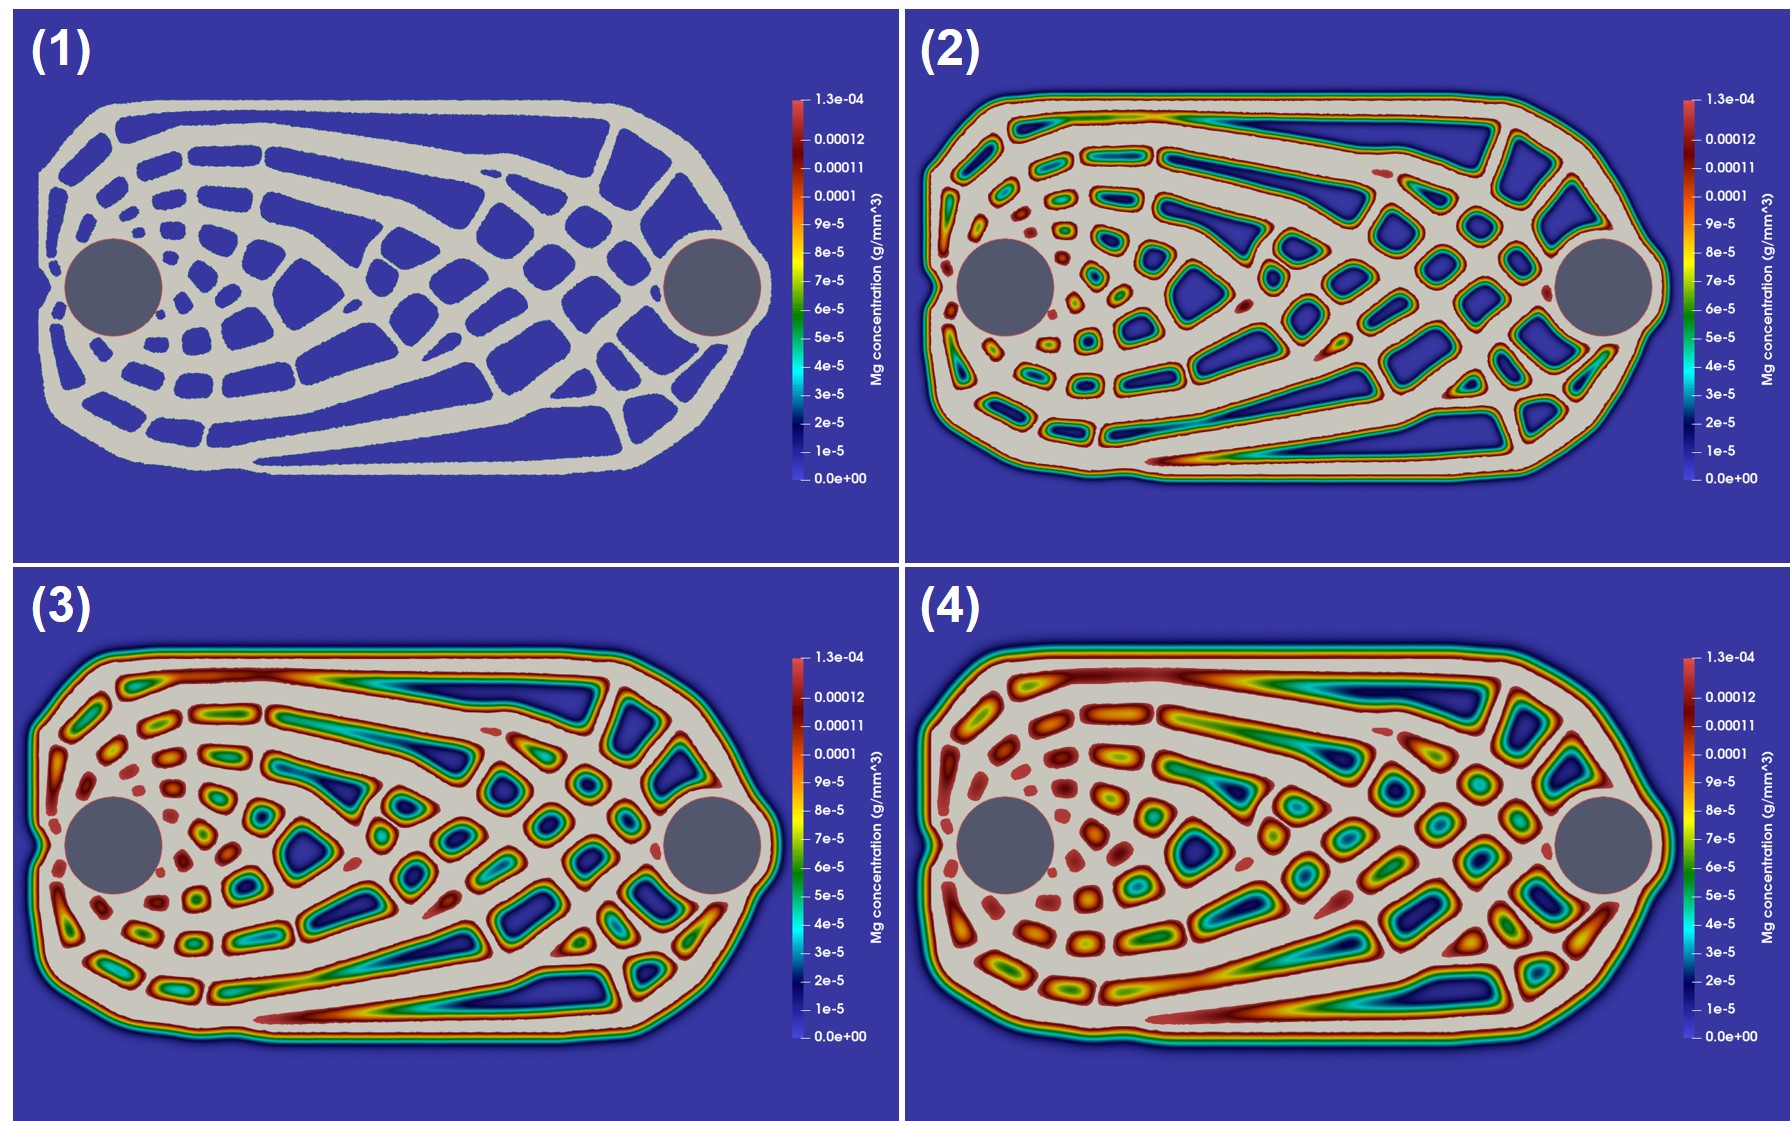
\includegraphics[width=\textwidth]{results_degradation_case1.jpg}
\caption[Visualization of the results of the biodegradation simulation for case 1]{Visualization of the results of the biodegradation simulation for case 1, showing the degrading of the infilled structure and release of Mg ions over time. The colors depict the Mg ions concentration.} \label{fig:infill_results_degradation_case1}
\end{figure}


\begin{figure}[h]
\centering
\medskip
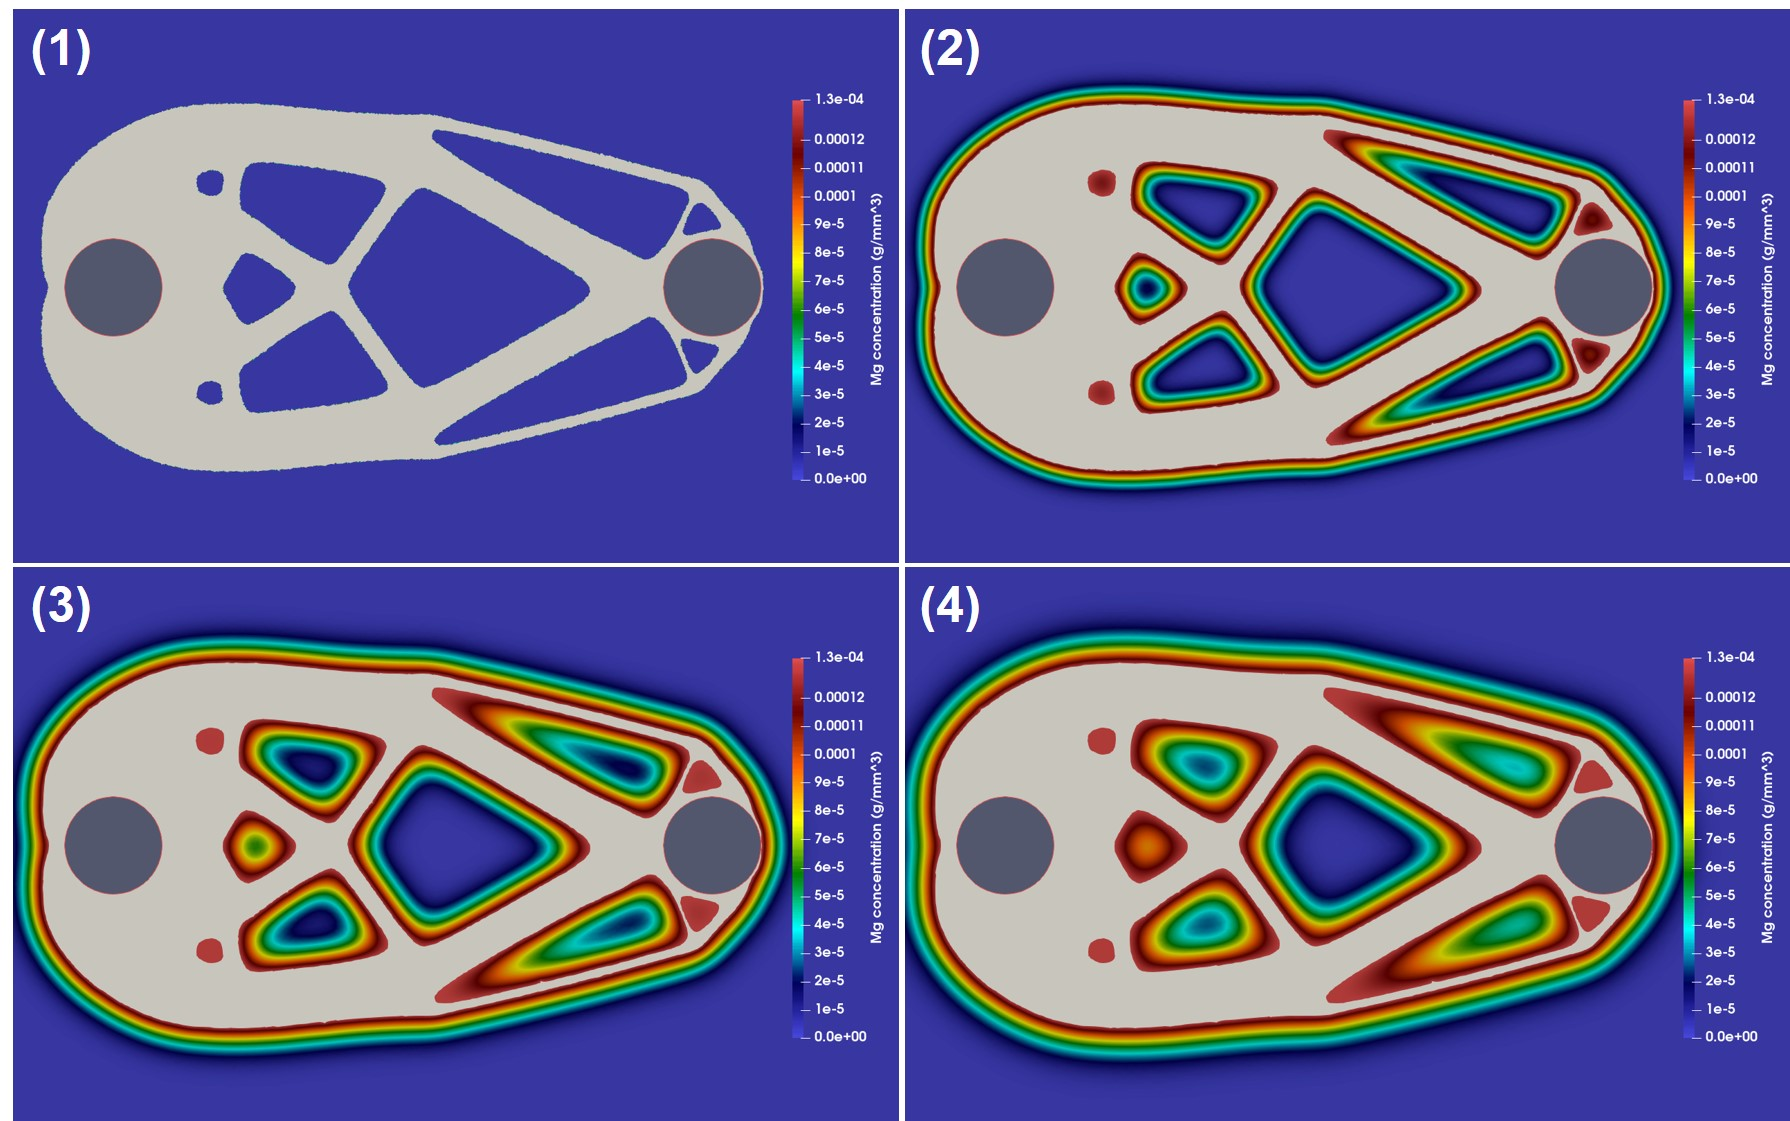
\includegraphics[width=\textwidth]{results_degradation_case2.jpg}
\caption[Visualization of the results of the biodegradation simulation for case 2]{Visualization of the results of the biodegradation simulation for case 2, showing the degrading of the infilled structure and release of Mg ions over time. The colors depict the Mg ions concentration.} \label{fig:infill_results_degradation_case2}
\end{figure}

As mentioned before, in order to increase the accuracy of the employed interface capturing method, the biodegradation model needs a refined mesh on the metal-environment interface. A closer look at the results of Fig. \ref{fig:infill_results_degradation_case1}, depicted in Fig. \ref{fig:infill_results_degradation_case1_zoom}, shows the mesh being refined on the interface. In this figure, the colors show the concentration of Mg ions released from the interface, and the biodegradation can be observed by the shrinkage of the light gray surface representing the undegraded parts of the infilled object.


\begin{figure}[h]
\centering
\medskip
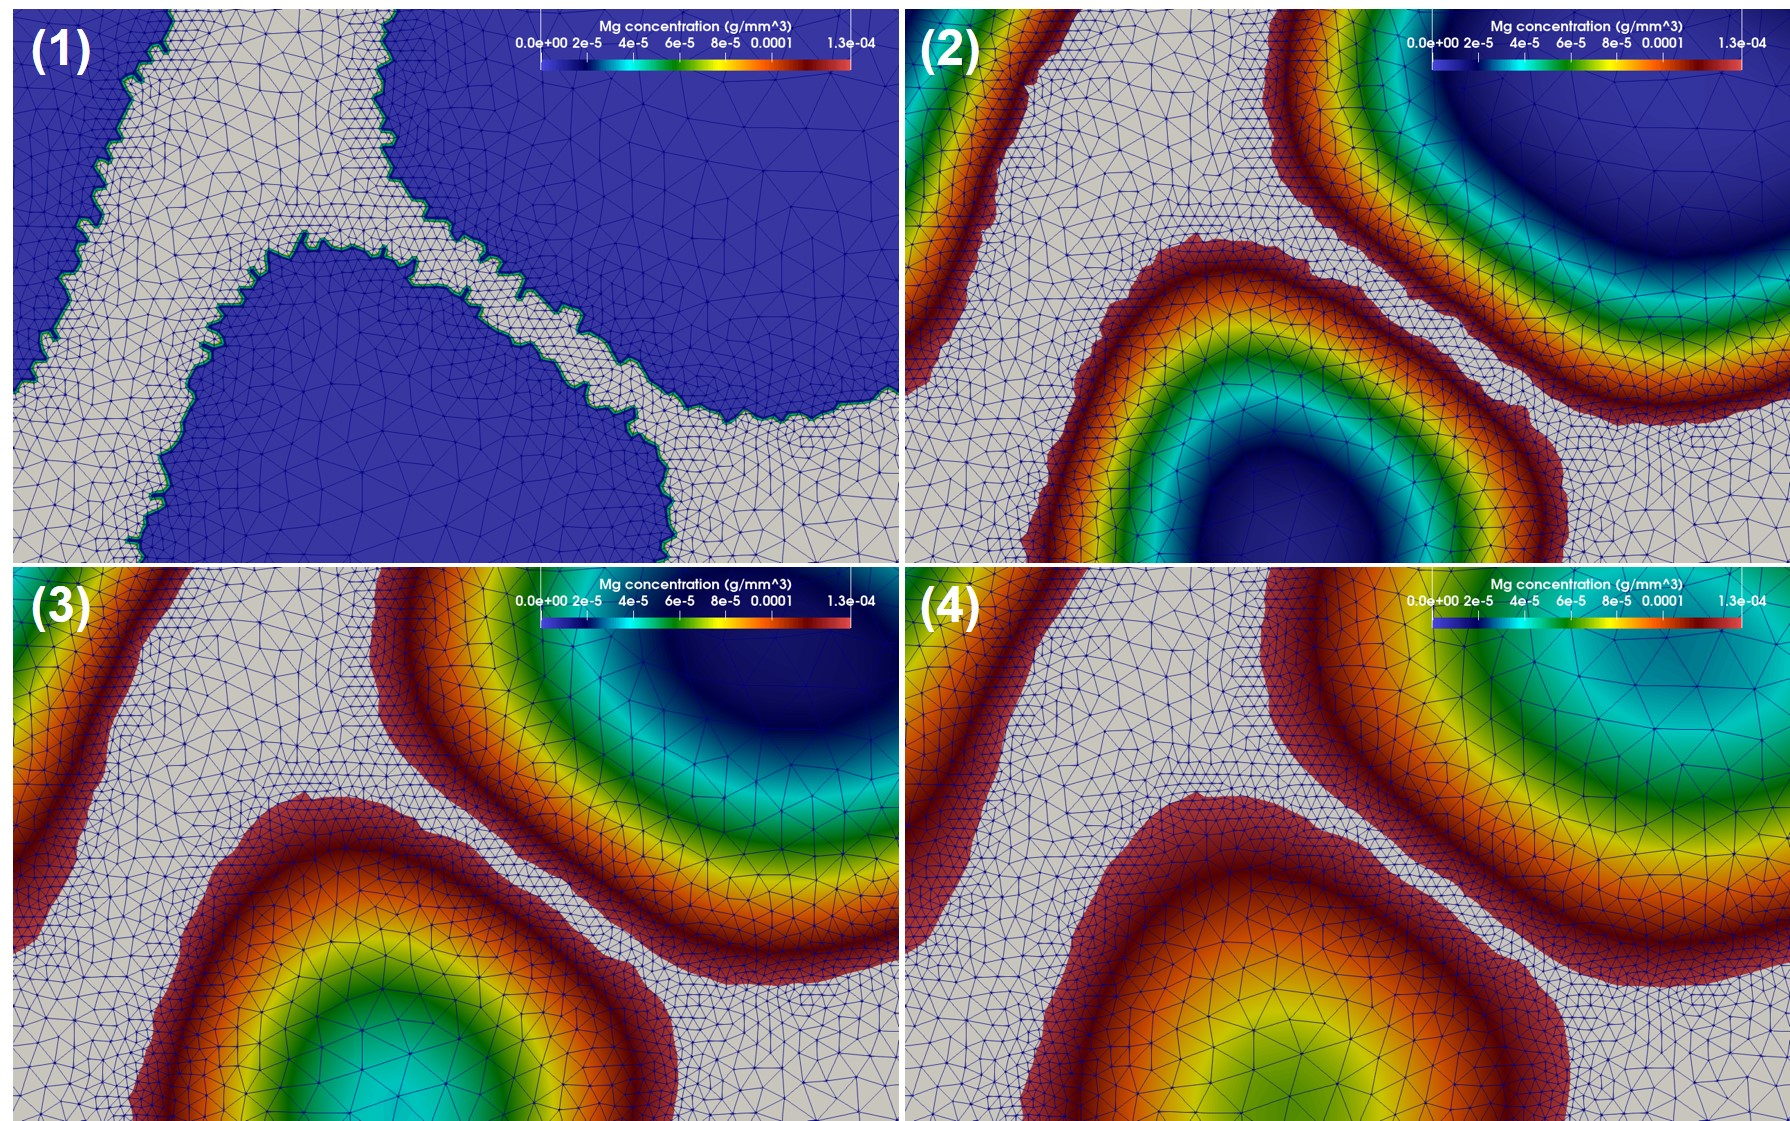
\includegraphics[width=\textwidth]{results_degradation_case1_zoom.jpg}
\caption[Zoom view of the results of the biodegradation simulation for case 1]{Zoomed view of the visualization results of the biodegradation simulation for case 1, showing the refined mesh, concentration of released ions, and shrinkage of the degrading object.} \label{fig:infill_results_degradation_case1_zoom}
\end{figure}

\section{Discussion}


%%%%%%%%%%%%%%%%%%%%%%%%%%%%%%%%%%%%%%%%%%%%%%%%%%
% Keep the following \cleardoublepage at the end of this file, 
% otherwise \includeonly includes empty pages.
\cleardoublepage

